\chapter{Evaluation}
\label{chapter:evaluation}

In this chapter, I introduce the setup I used for evaluating my visual question answering (VQA) model architecture. I describe important details about the GQA dataset \cite{hudson2019gqa}, analysing its composition and highlighting important points to consider when evaluating model performance. Next, I introduce a variety of baseline and state-of-the-art VQA models, summarising their primary features. I present results for these VQA architectures in \sectionautorefname{ \ref{section:performance_evaluation}}. Finally, I provide a detailed description of the hyperparameters of each of the components in my VQA architecture to aid the reproduction of my results.

\section{Datasets}

Whilst there are plenty of available datasets for visual question answering, I focus on just one for performance evaluation in this dissertation. I use the GQA dataset to evaluate the effectiveness of my VQA model architecture for three primary reasons. Firstly, it the only dataset that supports additional visual reasoning metrics such as validity, plausibility and distribution, as detailed in \subsectionautorefname{ \ref{subsec:visual_reasoning_metrics}}. Secondly, the GQA dataset is large in sample and vocabulary size and contains a balanced subset which deters models from exploiting statistical priors in question types and answer distributions, as described in \subsectionautorefname{ \ref{subsec:lanauge_priors_in_vqa_datasets}}. This makes it a suitable benchmark for evaluating the reasoning capabilities of VQA models when combined with the compositional nature of its questions. Finally, the GQA dataset contains scene graph annotations for its training and validation sets. Whilst other datasets contain scene graph annotations, these scene graphs are either too limited in their object, attribute and relationship vocabulary (\textit{e.g.} CLEVR \cite{johnson2017clevr} with 3 unique objects, 5 unique relations and 12 unique attributes), or their object, attribute and relationship vocabulary is extremely large (\textit{e.g.} Visual Genome (VG) \cite{krishna2017visual} with 75,729 unique objects, 40,480 unique relationships and 40,513 unique attributes). Instead of manually normalising the vocabulary of VG scene graphs and using VG to evaluate my model architecture, it is wiser to leverage GQA scene graphs, which are derived from VG scene graphs and comprise an already normalised vocabulary of 
1740 unique objects, 620 unique attributes and 330 unique relations.

% All Questions:
% 14305356 train, 2011853 val, 1340048 test, 172174 testdev, 713449 challenge

% Balanced Questions:
% 943000 train, 132062 val, 95336 test, 12578 testdev, 50726 challenge

% Image splits:
% 74942 train, 10696 val


In total, the GQA dataset comprises 22M question-image pairs, with 113M unique images. These question-image pairs are distributed across the training, validation, testing, development testing (test-dev) and challenge splits, ensuring that all question-image pairs with the same image are included in the same split. In total, the full training set contains around 77.1\% of all question-image pairs, the validation set contains 10.8\%, the test set 7.2\%, test-dev set 0.9\% and challenge set 3.8\%. The balanced portion of the GQA is much smaller, as many questions were omitted to smooth question type and answer distributions as detailed in \subsectionautorefname{ \ref{subsec:lanauge_priors_in_vqa_datasets}}. As a result, the balanced training, validation, test, test-dev and challenge sets contain 943,000, 132,062, 95,336, 12,578 and 50,726 question-image pairs respectively. Most importantly, the GQA dataset contains publicly-available scene graph annotations for the full train and validation sets, but not for the test, test-dev or challenge sets. Consequently, for all results and ablations, I train models on the balanced training set, I use the first half of the balanced validation set for hyperparameter optimisation, and use the second half of the balanced validation set as a test set.

The full GQA dataset has a total vocabulary size of 3,097 words, and an answer vocabulary of 1,878. The scene graphs (including those not available to the public) span a total of 1740 unique objects, 620 unique attributes and 330 unique relations. On average, the scene graph for each image contains 16-17 different objects, possibly with the same label. Additionally, each object is is related to an average of 3 other objects, and is associated with an average of 0.5 attributes. In reality, we typically see multiple attributes for more salient objects in the image, and none for less prominent objects.

Moreover, more salient objects tend to be more common in GQA scene graphs overall, since the original VG scene graphs were annotated by humans, whose eyes are naturally drawn towards more salient objects in images. As illustrated in \figureautorefname{ \ref{fig:gqa_scene_graph_object_relation_attribute_distribution}}, large objects like \textit{window, man, tree, building, etc.} tend to be more common than less salient objects or parts of objects like \textit{ear} and \textit{eye}.

\begin{figure}[htbp]
    \centering
    \begin{subfigure}[l]{0.33\textwidth}
        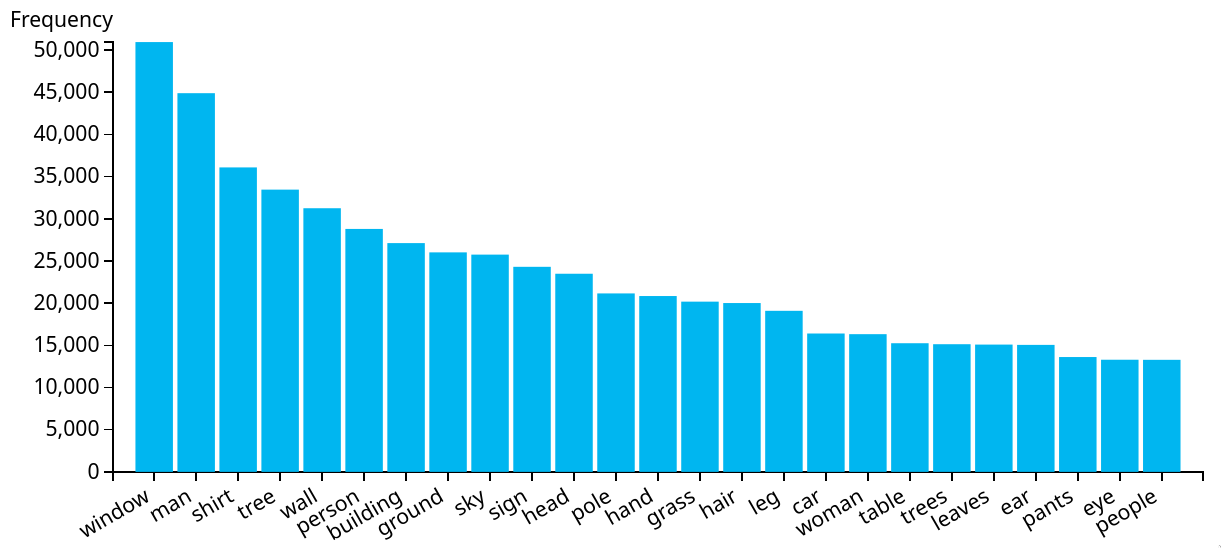
\includegraphics[width=\textwidth]{gqa_top_objects.png}
        \label{fig:gqa_top_objects}
        \caption{Top 25 GQA objects.}
    \end{subfigure}
    \begin{subfigure}[c]{0.32\textwidth}
        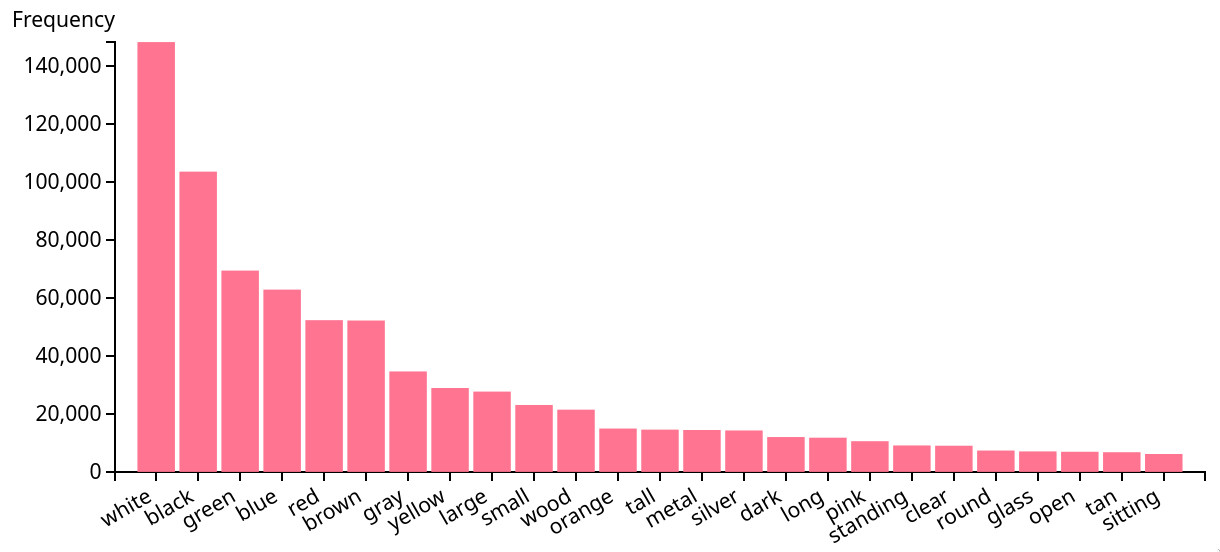
\includegraphics[width=\textwidth]{gqa_top_attributes.png}
        \label{fig:gqa_top_attributes}
        \caption{Top 25 GQA attributes.}
    \end{subfigure}
    \begin{subfigure}[r]{0.33\textwidth}
        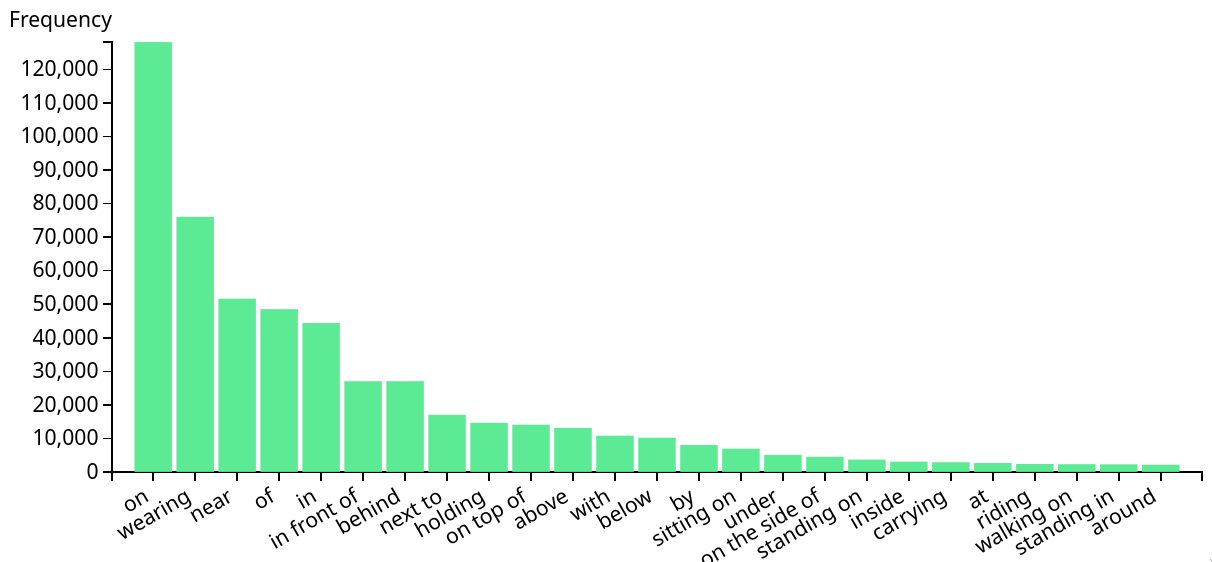
\includegraphics[width=\textwidth]{gqa_top_relations.png}
        \label{fig:gqa_top_relations}
        \caption{Top 25 GQA relations, excluding left and right.}
    \end{subfigure}
    \caption[An overview of GQA object, attribute and relation distributions.]{An overview of the objects, attributes and relations present in the GQA scene graphs, sorted by frequency. Figures are sourced from the GQA dataset website \cite{hudson2019gqa_website}.}
    \label{fig:gqa_scene_graph_object_relation_attribute_distribution}
\end{figure}

The majority of the most common attributes found in GQA scene graphs are colours. Some size-related attributes such as \textit{large, small, tall} and \textit{long} appear frequently as well, in addition to material-related attributes like \textit{wood} and \textit{glass}.

The most common scene graph relations in the GQA dataset are \textit{to the left of} and \textit{to the right of}, and have been excluded from the list of top relations to avoid dwarfing other relation types. Spatial relations like \textit{on, near, in, in front of, behind, next to, etc.} are the most common, but semantic relations containing verbs like \textit{holding, sitting, standing, carrying, riding} also comprise a large percentage of total relation types.

Despite the large variation in object, attribute and relation frequencies between different types displayed in \figureautorefname{ \ref{fig:gqa_scene_graph_object_relation_attribute_distribution}}, it is essential to note that the GQA dataset's balancing process accounts for both the question type and the subject of the question as described in \sectionautorefname{ \ref{section:vqa_datasets}}. For example, in the full GQA dataset, it might be reasonable to assume that questions about the material of a \textit{table} will have the answer \textit{wood} more often than less common materials like \textit{metal} or \textit{glass}. To create the balanced GQA subset, a subset of all questions about the material of a \textit{table} are chosen so that less common materials are more common in the answer distribution. As a result, even though attributes like \textit{metal} or \textit{glass} are less common than \textit{wood} in GQA scene graphs as a whole, the questions that ask about these attributes are more balanced in their answer distributions. This encourages VQA models to learn to identify and reason about less common scene graph objects, attributes and relations, and is one of the primary reasons why I choose to train my VQA model on the balanced portion of the GQA dataset instead of the full, unbalanced dataset.

To aid the evaluation of a VQA model's reasoning capabilities on different types of questions, every question in the GQA dataset is labelled as either \textit{open} or \textit{binary}, and is annotated with a semantic and a structural type. There are five structural types (query, compare, choose, logical and verify), and five semantic types (global, object, attribute, relation and category). I provide some example questions with various structural and semantic type combinations in \tableautorefname{ \ref{table:gqa_question_samples}}.

\begin{table}[htbp]
    \centering
    \begin{footnotesize}
    \begin{tabularx}{\linewidth}{cccL}
        \toprule
        \textbf{Type} & \textbf{Structural} & \textbf{Semantic} & \textbf{Example Question}\\
        \midrule
        % queryGlobal
        Open & Query & Global & How is the weather in the image?\\
        % % chooseGlobal
        % Open & Query & Global & Is it sunny or cloudy?\\
        % queryAttr
        Open & Query & Attribute & What color is the apple?\\
        % queryRel
        Open & Query & Relation & What is the small girl wearing?\\
        % queryObject
        Open & Query & Category & What kind of fruit is on the table?\\
        % chooseAttr
        Open & Choose & Attribute & Is the apple green or red?\\
        % chooseRel
        Open & Choose & Relation & Is the cat to the left or to the right of the flower?\\
        % chooseObjRel
        Open & Choose & Relation & What is the boy eating, an apple or a slice of pizza?\\
        % chooseObject
        Open & Choose & Category & What kind of fruit is it, an apple or a banana?\\
        % common
        Open & Compare & Object & What is common to the shirt and the flower?\\
        % verifyGlobal
        Binary & Verify & Global & Is it cloudy today?\\
        % exist
        Binary & Verify & Object & Is there an apple in the picture?\\
        % verifyAttr
        Binary & Verify & Attribute & Is the apple red?\\
        % % existRel
        % Binary & Verify & Relation & Is there an apple on the black table?\\
        % verifyRel
        Binary & Verify & Relation & Is she wearing a blue dress?\\
        % logicOr
        Binary & Logical & Object & Do you see either an apple or a banana there?\\
        % verifyAttrs
        Binary & Logical & Attribute & Is the apple red and shiny?\\
        % logicAnd
        Binary & Logical & Object, Attribute & Do you see both green apples and bananas there?\\
        % % compare
        % Binary & Compare & Object & Who is taller, the boy or the girl?\\
        % twoSame
        Binary & Compare & Object & Does the shirt and the flower have the same color?\\
        % % twoDiff
        % Verify & Compare & Object & Are the table and the chair made of different materials?\\
        % % allSame
        % Verify & Compare & Object & Are all the people there the same gender?\\
        % % allDiff
        % Verify & Compare & Object & Are the animals in the image of different types?\\
        \bottomrule
    \end{tabularx}
    \caption{A selection of questions from the GQA dataset and their corresponding semantic and structural types, adapted from the GQA supplementary material \cite{hudson2019gqa_preprint}.}
    \label{table:gqa_question_samples}
    \end{footnotesize}
\end{table}

As seen in \tableautorefname{ \ref{table:gqa_question_samples}}, binary question types can always be answered with either \textit{yes} or \textit{no}, where \textit{open} question types require answering with one of the 1,878 concepts in the GQA answer vocabulary. Naturally, I would expect that most models would perform better on binary questions than open questions.

Inspecting structural types, we see that the \textit{query} and \textit{choose} structural types only apply to \textit{open} questions, as they require answering with an object, relation or attribute from the image, rather than with \textit{yes} or \textit{no}. The \textit{compare} structural type is applicable to both binary and open questions, depending on question phrasing; open comparisons usually require reasoning about what is the same or different between two objects, where binary comparisons only require identifying if a certain property is the same or different. Finally, the \textit{verify} and \textit{logical} structural types apply to binary questions, as they aim to determine whether a specific combination of object, relationships and/or attributes exists.

The semantic type of a question is related to its subject; questions belonging to the \textit{global} semantic type ask about properties of the image as a whole instead of individual objects, attributes and relations. Conversely, questions belonging to the \textit{object}, \textit{attribute} or \textit{relation} semantic type naturally query about object, attributes and/or relations in the scene. Interestingly, the \textit{category} semantic type is only applicable to \textit{open}-type questions, as they require the a VQA model to identify that an object is part of a certain category, \textit{e.g.} that an \textit{apple} is a type of fruit. Converting the question \textit{What kind of fruit is on the table?} to a binary question would result in a question like \textit{Is the apple on the table a kind of fruit?}, which doesn't require a visual signal to answer effectively.

I delve into the semantic and structural question type distributions for the portion of the GQA dataset used for result collection in \sectionautorefname{ \ref{sec:ablation_studies}}, as it is important to consider when comparing model performance on different types of questions.

From the dataset analysis above, there are a few hypotheses that we can make about how my model might perform for various question types:

\begin{enumerate}
    \item Given that binary questions are generally easier to answer than open questions, we should see a higher accuracy on binary questions than open-type questions for my model architecture and variations thereof.
    \item Since my model architecture only uses object, attribute and relation scene graph information as its visual signal, we should see lower performance on questions belonging to the \textit{global} semantic when compared to questions belonging to the \textit{object}, \textit{attribute} or \textit{relation} semantic types.
    \item My model should perform well on questions belonging to the \textit{verify} or \textit{logical} structural types, as they mostly require reasoning over a localised neighbourhood of object, relations and attributes, and are only applicable to binary question types.
\end{enumerate}

I will discuss these hypotheses in detail in \sectionautorefname{ \ref{sec:ablation_studies}}.

\section{Baselines}

To gain a better understanding of how my well my model architecture performs on the GQA dataset, I compare it to a variety of current baseline and state-of-the-art methods in \chapterautorefname{ \ref{chapter:results}}. To understand why some models perform better than others, I introduce these baseline VQA models in this section, summarising their key components and highlighting the type of visual data that they use for the VQA task.

\textbf{LXMERT} \cite{tan2019lxmert}: Motivated by the success of transformer-based models \cite{vaswani2017attention} for Natural Language Processing (NLP) tasks, \citeauthor{tan2019lxmert} built LXMERT for learning general multi-modal representations. In the context of VQA, the LXMERT model uses two self-attention transformer encoders and one cross-modality transformer encoder. The first self-attention encoder is responsible for attending to Faster R-CNN \cite{ren2016faster} and bounding box features, and the second second is a language encoder, which attends to word features. The outputs of these encoders are fed to the cross-modality encoder, which employs a bi-directional attention flow between the visual and textual encodings to align the two modalities, followed by separate self-attention layers to allow the model to attend to any newly-discovered important features after multi-modal alignment.

\textbf{Bilinear Attention Networks (BAN)} \cite{kim2018bilinear}: In the context of VQA, co-attention methods capture which parts of the question are important given the visual signal as a whole, and vice versa. Bilinear attention methods capture which parts of the question are important given each feature of the visual signal and vice-versa, making them much more expressive, but computationally expensive. \citeauthor{kim2018bilinear} build upon low-rank bilinear modelling techniques \cite{wolf2007modeling, pirsiavash2009bilinear} to approximate bilinear interactions between textual and visual input signals as follows:

Given a matrix of question features \(Q \in \R^{n_Q \times d_Q}\) and a matrix of visual features \(R \in \R^{n_R \times d_R}\), BAN learns a bilinear attention map \(\mathcal{A} \in \R^{d_Q \times d_R}\), where each pre-softmax entry of \(\mathcal{A}\) is defined as \(\mathcal{A}_{ij} = p^\top((U^\top Q_i) \circ (V^\top R_j))\), where \(U \in \R^{d_Q \times k}\) and \(V \in \R^{d_R \times k}\) are projection matrices that project \(Q\) and \(R\) respectively onto a common dimension and \(p \in \R^{k}\) pools the elements of \((U^\top Q_i) \circ (V^\top R_j)\) into a single value.

For each attention map \(\mathcal{A}\), BAN creates a joint embedding of \(Q\) and \(R\), \(f \in \R^C = \text{BAN}(Q, R; \mathcal{A}) = P^\top f'\) where \(P \in \R^{K \times C}\) is a pooling matrix that combines intermediate joint features \(f'\). Each element of \(f'\) models a bilinear combination of projected input features \(\sigma (Q^\top U')\) and \(\sigma (R^\top V')\), using \(\mathcal{A}\) as a bilinear weight matrix, \textit{i.e.} \(f'_k = \sigma (Q^\top U')^\top_k \cdot \mathcal{A} \cdot \sigma (R^\top V')_k\), where \(\sigma\) is some non-linear acrivation function.

To show the effectiveness of the joint representation \(f\), the authors collect multiple bilinear attention maps \textit{(glimpses)} and combine their respective joint features using residual learning techniques \cite{kim2016multimodal}, achieving state-of-the-art results on the VQAv2 dataset in \citeyear{kim2018bilinear}. In their final model, the authors use a matrix of Faster R-CNN object features as the visual representation \(R\), and Gated Recurrent Unit (GRU) \cite{cho2014learning} outputs as the question representation \(Q\).

\textbf{Graph Reasoning Networks (GRN)} \cite{guo2019bilinear}: GRNs improve on the BAN architecture by capturing relationships between BAN's default joint question-image representations and previously captured joint representations. Given a visual representation and a question representation, GRNs first compute a vector of joint question-image features, as in BAN. These multi-modal features are then projected back on to the question to yield an output representation for the layer, in an effort to determine which joint question-object representations are relevant to the original question. The authors repeat this process multiple times in an effort to promote multi-step reasoning; with each repetition, instead of using the original question representation for computing joint representations, subsequent joint features are computed using the previous layer's output.

% \textbf{Modular Co-Attention Networks (MCAN)} \cite{yu2019deep}:

\textbf{Mutual and Self Attention (MSA)} \cite{farazi2020attention}: The three primary inputs to the MSA model are a question representation \(q\), a visual representation \(v\) and a collection of semantic relationships \(r\). From these inputs, the MSA module computes eight attention distributions which it fuses together, four from \(q\) and \(r\), and four from \(q\) and \(v\). Taking \(q\) and \(r\) as an example, the MSA module computes the following:

\begin{itemize}
    \item The attention distribution over \(q\), guided by a fused representation of \(q\) and \(r\), called \textit{mutual attention}. This captures which part of the question are important to the combined question and relationship features.
    \item The attention distribution over \(r\), guided by a fused representation of \(q\) and \(r\). This captures which relationship features are important to the combined question and relationship embeddings.
    \item The attention distribution over \(q\), guided by self-attended question features \(\psi_{q, q}\). This emphasises the most important parts of the question.
    \item The attention distribution over \(r\), guided by a linear transformation of \(\psi_{r, q}\), where \(\psi_{r, q}\) is a multi-head attention distribution over \(r\), guided by \(q\). This emphasises relationship features that are deemed important to answering the question.
\end{itemize}

The authors achieve promising results with this setup using various combinations of features for \(r\) and \(v\), from Faster R-CNN and bounding box features to pre-annotated scene graph features from the GQA dataset.

\textbf{Compositional Attention Networks (MAC)} \cite{hudson2018compositional}: As introduced in \subsectionautorefname{ \ref{subsection:attention_methods_for_vqa}}, the compositional attention network is a widely accepted VQA baseline for the GQA dataset. Its recurrent cell design promotes decomposing a question into discrete reasoning steps, where two values are passed from cell to cell: The first is a control vector, responsible for determining which part of the question to attend to for a given reasoning step. The second is a memory vector, which contains the intermediate result of the current reasoning process. As originally implemented for the GQA dataset, the compositional attention network relies on a BiLSTM-encoded question representation and a knowledge-base of Faster R-CNN \cite{ren2016faster} object features as its visual signal, however its knowledge-base is easily replaced with scene graph features as discussed in \sectionautorefname{ \ref{section:performance_evaluation}}.

% \begin{table}[htbp]
%     \begin{footnotesize}
%         \begin{tabularx}{\linewidth}{@{}lCccCcCC@{}}
%             \toprule
%             \multirow{2}{*}{\textbf{Model}} & \multicolumn{7}{c}{GQA Test-standard} \\
%             \cmidrule{2-8}
%             & Accuracy & Binary & Open & Consistency & Validity & Plausibility & Distribution \\
%             \midrule
%             Human \cite{hudson2019gqa} & 89.30 & 91.20 & 87.40 & 98.40 & 98.90 & 97.20 & - \\
%             \midrule
%             Global Prior \cite{hudson2019gqa} & 28.90& 42.94 & 16.62 & 51.69 & 88.86 & 74.81 & 93.08\\
%             Local Prior \cite{hudson2019gqa} & 31.24 & 47.90 & 16.66 & 54.04 & 84.33 & 84.31 & 13.98\\
%             LSTM \cite{hudson2019gqa} & 41.07 & 61.90 & 22.69 & 68.68 & 96.39 & 87.30 & 17.93\\
%             CNN \cite{hudson2019gqa} & 17.82 & 36.05 & 1.74 & 62.40 & 35.78 & 34.84 & 19.99\\
%             LSTM + CNN \cite{hudson2019gqa} & 46.55 & 63.26 & 31.80 & 74.57 & 96.02 & 84.25 & 7.46\\
%             \midrule
%             Bottom-Up \cite{anderson2018bottom} & 49.74 & 66.64 & 34.83 & 78.71 & 96.18 & 84.57 & 5.98\\
%             MAC \cite{hudson2018compositional} & 54.06 & 71.23 & 38.91 & 81.59 & 96.16 & 84.48 & 5.34\\
%             BAN \cite{kim2018bilinear} & 57.10 & 76.00 & 40.41 & 91.70 & 96.16 & 85.58 & 10.52\\
%             LXMERT \cite{tan2019lxmert} & 60.33 & 77.16 & 45.47 & 89.59 & 96.35 & 84.53 & 5.69\\ % val 59.80%, 60.00% test-dev
%             TRRNet \cite{yangtrrnet} & 60.74 & 77.83 & 45.65 & 90.95 & 96.40 & 85.15 & -\\
%             GRN \cite{guo2019bilinear} & 61.22 & 78.69 & 45.81 & 90.31 & 96.36 & 85.43 & 6.77\\
%             NSM \cite{hudson2019learning} & 63.17 & 78.94 & 49.25 & 93.25 & 96.41 & 84.28 & 3.71\\
%             TRRNet\(^*\) \cite{yangtrrnet} & 63.20 & 77.91 & 50.22 & 89.84 & 96.47 & 85.15 & 5.25 \\
%             \midrule
%             LXMERT\(^\dagger\) \cite{tan2019lxmert} & 62.71 & 79.79 & 47.64 & 93.1 & 96.36 & 85.21 & 6.42\\
%             NSM\(^\dagger\)	& 67.55 & 80.45 & 56.16 & 93.83 & 96.53 & 84.16 & 2.78\\
%             HAN\(^{\dagger*}\)\cite{kim2020hypergraph} & 73.33 & 79.68 & 67.73 & 77.02 & 96.36 & 83.70 & 2.46\\
%             TRRNet\(^{\dagger*}\) \cite{yangtrrnet} & 74.03 & 82.12 & 66.89 & 89.00 & 96.76 & 83.58 & 1.29\\
%             \bottomrule
%         \end{tabularx}
%         \caption[Baseline and state-of-the-art VQA model performance on the GQA test-standard set]{A comparison of various models on the GQA test set for multiple metrics, including top models from the GQA challenge leaderboard \cite{gqachallenge} for which results have been formally published. Models marked with a \(^*\) use scene graph and/or functional program annotations during training, and those marked with a \(^\dagger\) are ensemble models.}
%     \end{footnotesize}
% \end{table}

% Where possible, I source GQA validation set scores for a variety of GQA models. In general, we see improvements of up to 



% 73.65 MAC + object, attribute, relation identities.

% \cite{guo2019bilinear}
% BAN-4 × 1 44.8M 61.95
% BAN-4 × 2 79.4M 62.60
% BAN-4 × 3 115.8M 61.98
% Inter × 1 32.9M 61.88
% Inter × 1 + Intra × 1 51.8M 63.50
% Inter × 1 + Intra × 2 70.7M 63.80
% Inter × 1 + Intra × 3 89.6M 63.60
% (Inter + Intra) × 2 96.9M 64.07
% (Inter + Intra) × 3 142.1M 64.22


\section{Implementation Details}

In this section, I provide relevant details about the implementation of my architecture, from its vocabulary construction through to its parameter configuration and optimisation method. I refer the reader to \chapterautorefname{ \ref{chapter:methodology}} for model-specific nomenclature used in this section, and to \appendixautorefname{ \ref{appendix:resources}} for the source code used to collect all results.

Since my model architecture uses only the train and validation sets, I build a question vocabulary of 2,912 case-sensitive words, and a scene graph vocabulary of \(|S_o| = 1703\) unique objects, \(|S_a| = 617\) unique attributes and \(|S_r| = 310\) unique relations using the combined train and validation questions and scene graph annotations respectively. Moreover, the output module of my architecture predicts an answer from one of 1,842 possible answers in the combined balanced train and validation sets, slightly less than the 1,878 answers in the full GQA set.

In both the question and scene graph embedding modules, I use \(d_{H_q} = d_{H_r} = 300\)-dimensional GloVe vectors \cite{pennington2014glove} to embed all words. In the event where a question token or scene graph object, attribute or relation comrises multiple words \textit{e.g. to the right of}, I represent that token as an average of the GloVe embeddings of its individual words.

The question processing module is a single-layer bi-directional LSTM \cite{hochreiter1997long} with input dimension \(d_{H_q} = 300\). Each direction of the BiLSTM has a hidden dimension of \(\frac{d_{K_q}}{2}\), where \(d_{K_q} = 256\) is the dimension of each token in the question knowledge-base \(K_q\). To avoid processing the vectors used for padding and consequently ruining question embeddings, I use PyTorch's inbuilt \texttt{pack\_squence} function. \cite{paszke2019pytorch}

The scene graph module is a three-layer graph attention network (GAT), with all attention computations as described in the original GAT publication \cite{velivckovic2017graph}. The first layer has an imput dimension of \(d_{H_r} = 300\) and an output dimension of \(d_{K_r} = 256\), and subsequent layers have input and output dimensions of \(d_{K_r} = 256\). Each layer has \(n_h = 4\) attention heads, the outputs of which are concatenated after each layer to maintain a constant layer size. No non-linear activation function is used to transform the outputs of each layer.

The compositional attention network used for the reasoning module has a length of 4, and a hidden dimension of 512 as described in the original paper \cite{hudson2018compositional}. As in the original implementation, I use ELU activations over ReLU in the control, read, write units, and all dropout layer probabilities are set to 0.15.

The output module is implemented according to the original implementation of the compositional attention network, again using ELU over ReLU for activation functions and dropout probabilities of 0.15. Naturally, the last linear layer of the output module has a dimension of 1,842, the same as the answer vocabulary size for the combined balanced GQA train and validation sets.

For optimisation, I use a standard categorical cross-entropy loss with an Adam optimiser \cite{kingma2014adam}. The optimiser uses standard exponential decay rates of \(\beta_1 = 0.9, \beta_2 = 0.999\) and an epsilon of \(\varepsilon = 10^{-8}\). I clip all gradients with a \(\ell_2\) norm greater than 8, as used by \citeauthor{hudson2018compositional} for their compositional attention network. All models are trained for 32 epochs with a batch size of 16 at a constant learning rate of \(4.7611 \times 10^{-5}\) (\textit{5 s.f.}).
